\documentclass{beamer}

\usepackage[utf8]{inputenc}
\usepackage[spanish]{babel}
\usepackage{booktabs, makecell, multirow}
\usepackage{graphicx}
\usepackage{tikz}
\usepackage{color, colortbl}
\usepackage[font=tiny,labelfont=bf, format=plain,justification=centering,labelformat=empty]{caption}
\usepackage{fontawesome6}
\usepackage{verbatim}
\usepackage{listings}
\lstset{basicstyle=\ttfamily\footnotesize, language=Bash}
\graphicspath{{./figures}}
\usetheme{CambridgeUS}

\renewcommand\theadfont{\bfseries} % bold tabular headers
\renewcommand\theadalign{ll}
\renewcommand\theadgape{}


\definecolor{mygray}{RGB}{100, 100, 100}
\definecolor{myred}{RGB}{175, 7, 31}
\setbeamercolor{palette primary}{bg=mygray,fg=myred}
\setbeamercolor{palette secondary}{bg=mygray!10!white,fg=myred}
\setbeamercolor{palette tertiary}{bg=myred,fg=white}
\setbeamercolor{block title}{bg=mygray, fg=black}
\setbeamercolor{block title alerted}{bg=myred, fg=white}
\setbeamercolor{block body}{fg=black,bg=mygray!10!white}
\setbeamercolor{block body alerted}{fg=black, bg=myred!10!white}
\setbeamerfont{block body}{size=\small}
\setbeamerfont{block body alerted}{size=\small}
\setbeamerfont{block body example}{size=\small}
\setbeamerfont{block title}{size=\small}
\setbeamerfont{block title alerted}{size=\small}
\setbeamerfont{block title example}{size=\small}
\hypersetup{
  colorlinks,
  allcolors=red,
  urlcolor=blue,
}
\setbeamercolor{section number projected}{bg=mygray,fg=myred}
\setbeamertemplate{itemize item}[triangle]
\setbeamercolor{itemize item}{fg=mygray}
\setbeamertemplate{itemize subitem}[circle]
\setbeamercolor{itemize subitem}{fg=myred!50!white}
\setbeamercolor{section in head/foot}{bg=myred!20!white, fg=mygray}


\title{Curso de Introducción a Git y GitHub}
\subtitle{Día 2 - Iniciación a Git}

\author{Héctor Nieto}

\institute{Instituto de Ciencias Agrarias, CSIC}
\date{2026}


\logo{
\includegraphics[height=0.5cm]{CSIC}}

\begin{document}

 \begin{frame}
  \titlepage
 \end{frame}

	\begin{frame}{Crear repositorios}
	 \begin{columns}
	  \begin{column}{0.6\linewidth}
	   \begin{itemize}
	    \item \texttt{git init}: Crea un repositorio git (vacío) en esa carpeta
	    \vspace{2cm}
	    \item \texttt{git clone <git\_URL>}: Clona (descarga) un respositorio remoto en esa carpeta
	   \end{itemize}
	  \end{column}
			\begin{column}{0.4\linewidth}
			 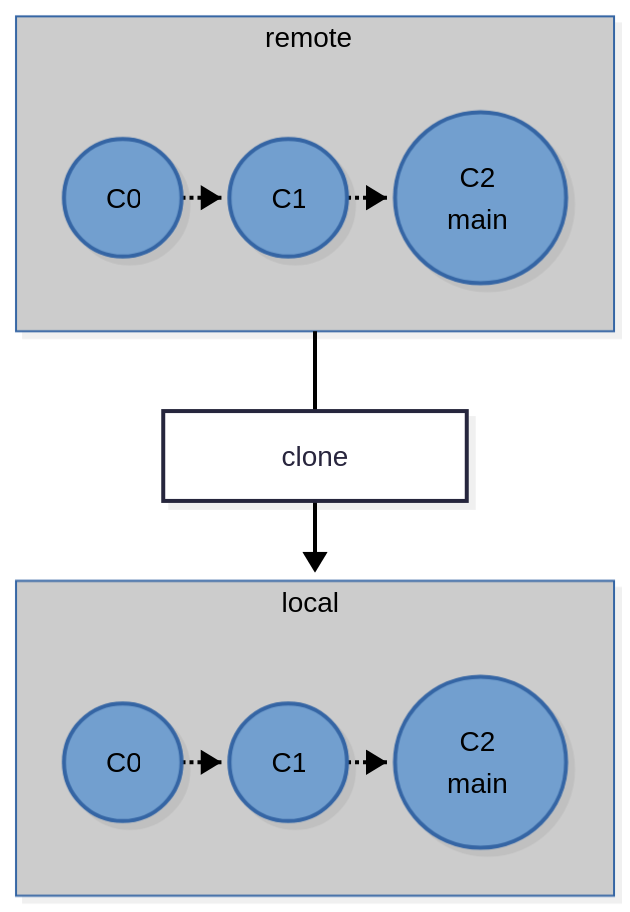
\includegraphics[width=\columnwidth]{02_clone}
		 \end{column}
	 \end{columns}
	\end{frame}


	\begin{frame}{Versionado}
	 \centering
	 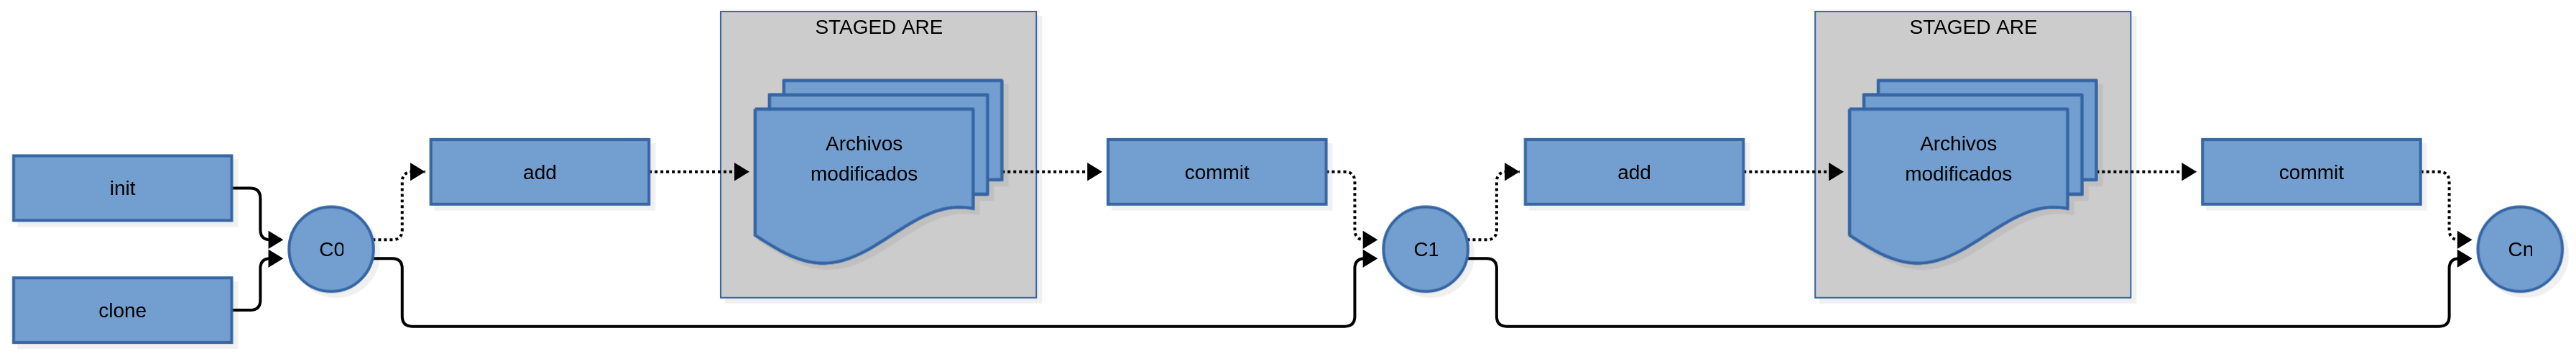
\includegraphics[width=\textwidth]{02_versionado}\\
	 \vspace{1cm}
	 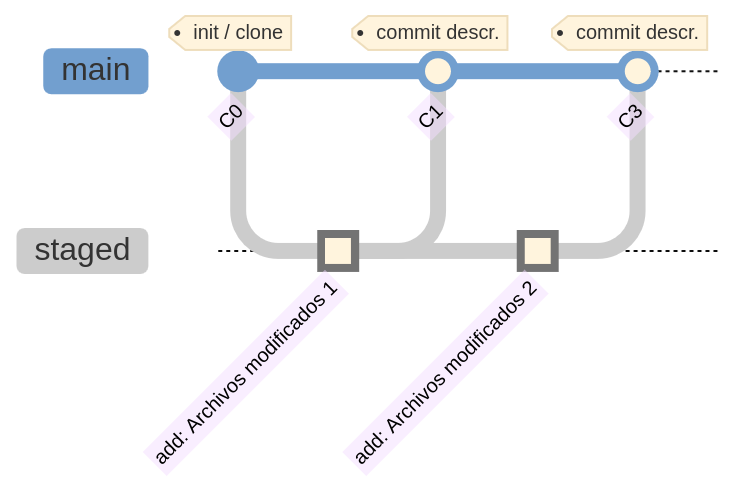
\includegraphics[width=0.5\textwidth]{02_git_commit}\\
	\end{frame}


	\begin{frame}{Control de cambios}
	 \centering
	 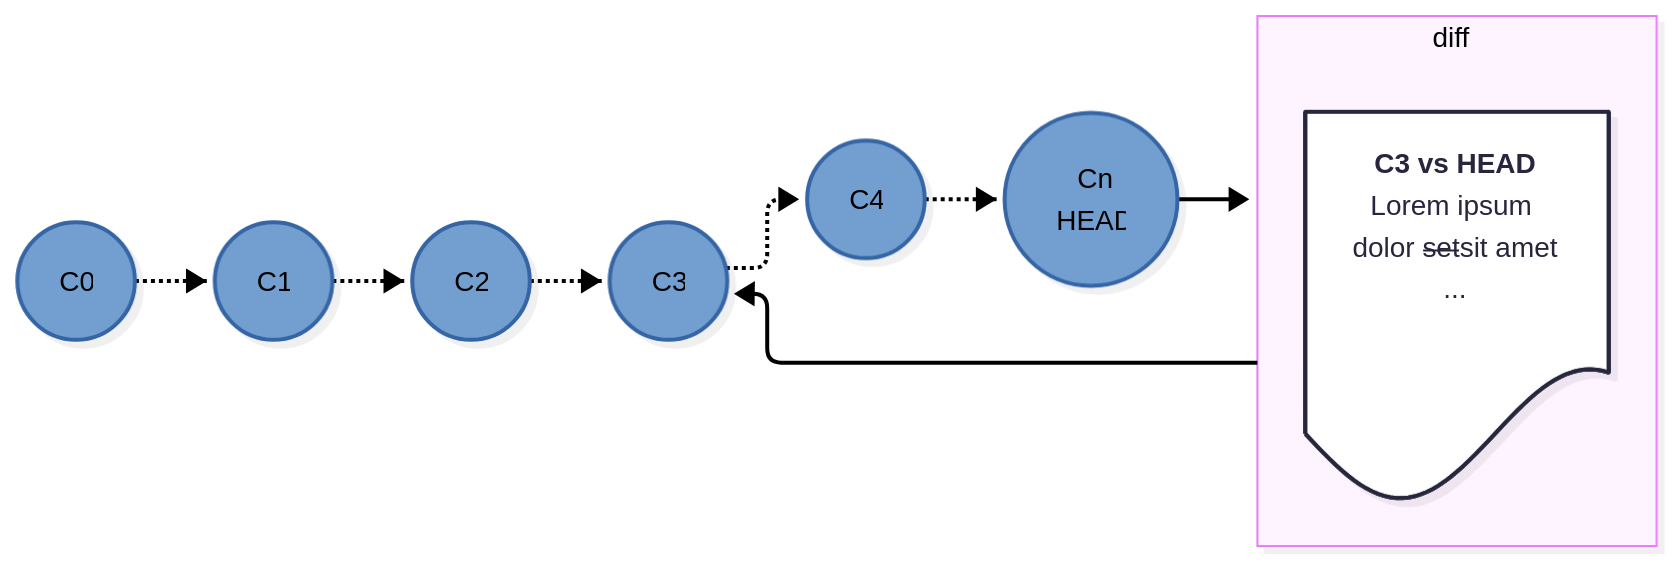
\includegraphics[width=\textwidth]{02_diff}\\
	 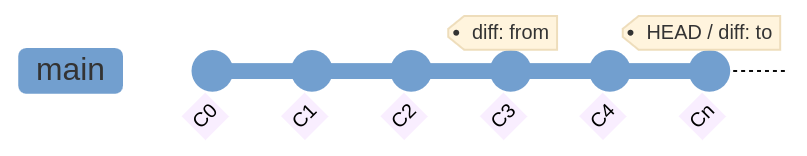
\includegraphics[width=\textwidth]{02_git_diff}
	\end{frame}


	\begin{frame}{Restaurado: checkout}
	 \centering
	 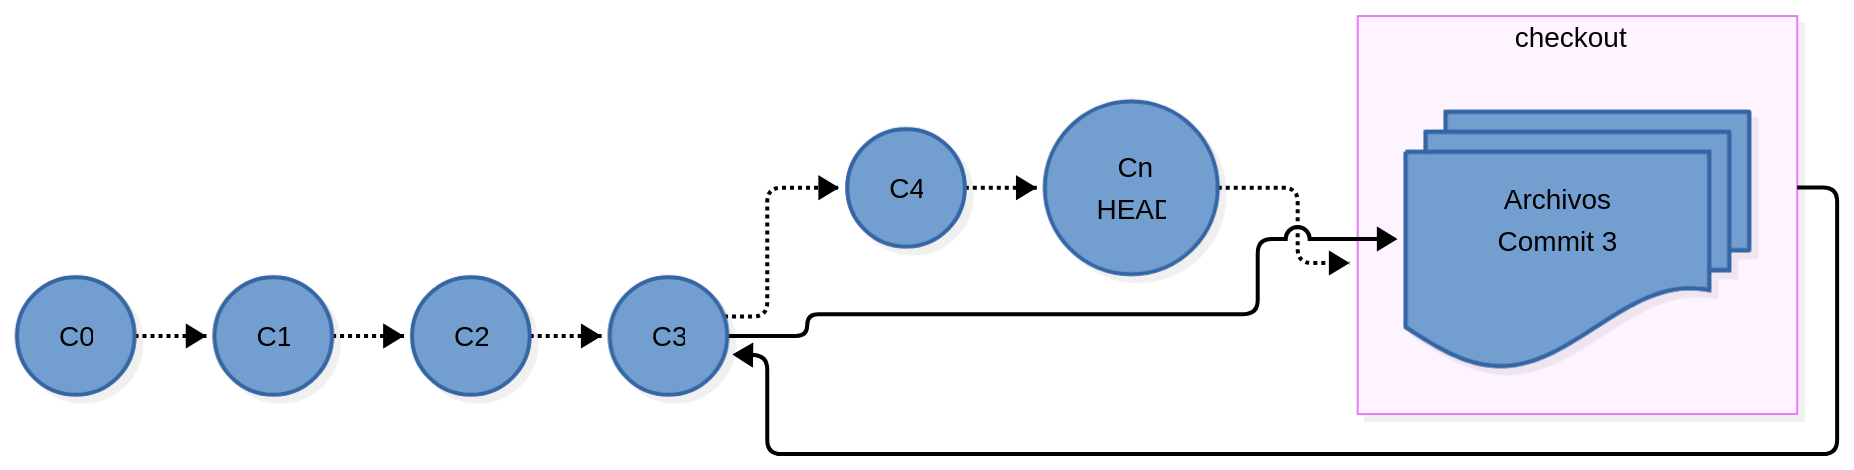
\includegraphics[width=\textwidth]{02_checkout}\\
	 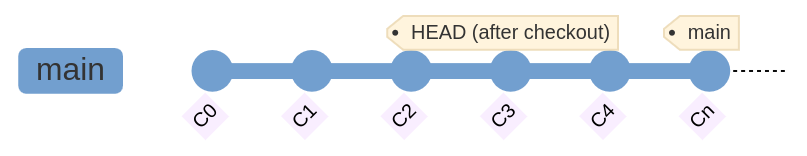
\includegraphics[width=\textwidth]{02_git_checkout}
	\end{frame}


	\begin{frame}{Restaurado: revert}
	 \centering
	 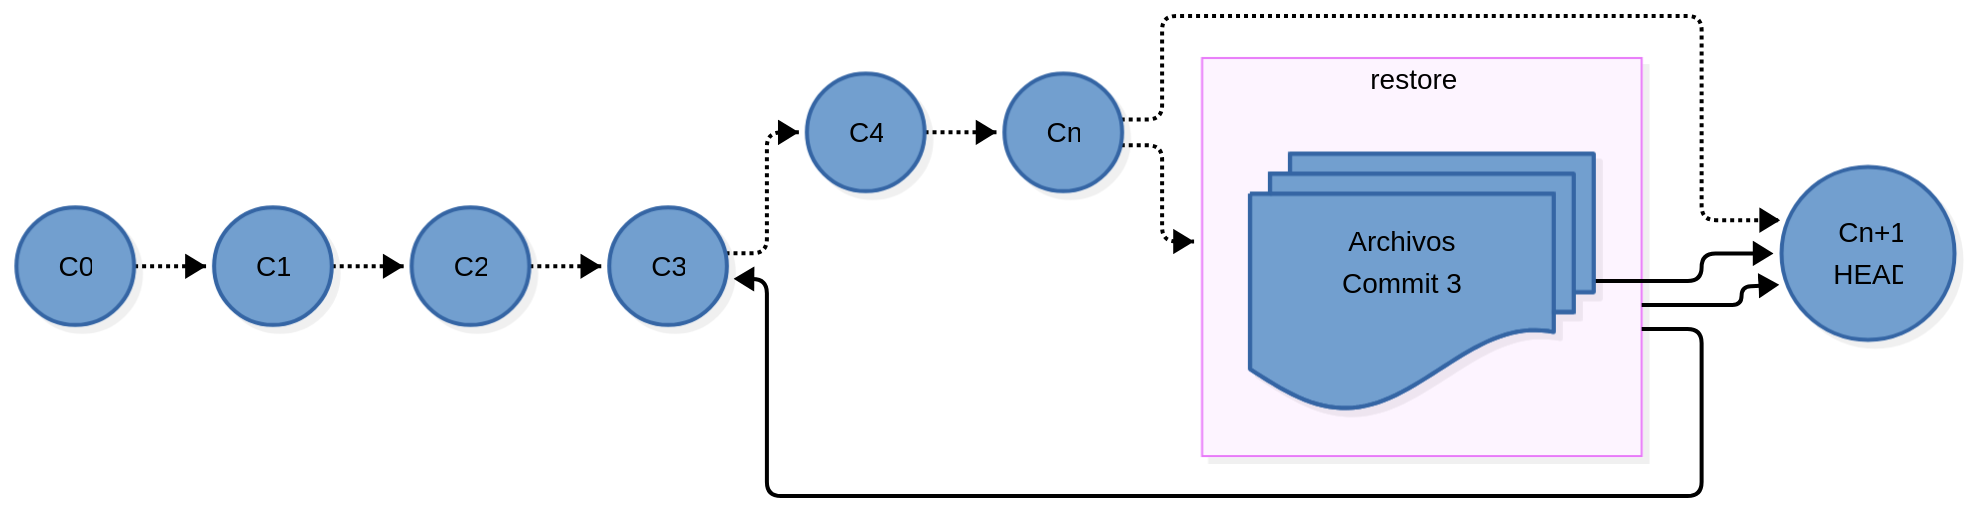
\includegraphics[width=\textwidth]{02_restore}\\
	 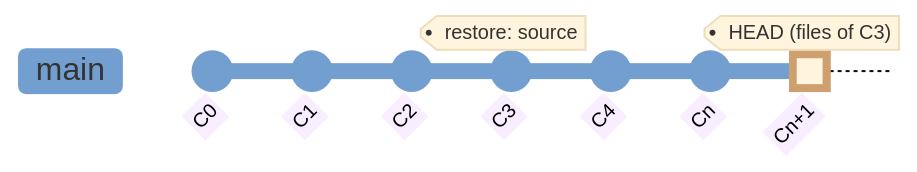
\includegraphics[width=\textwidth]{02_git_restore}
	\end{frame}


	\begin{frame}{Repositorio local y remoto}
	 \centering
	 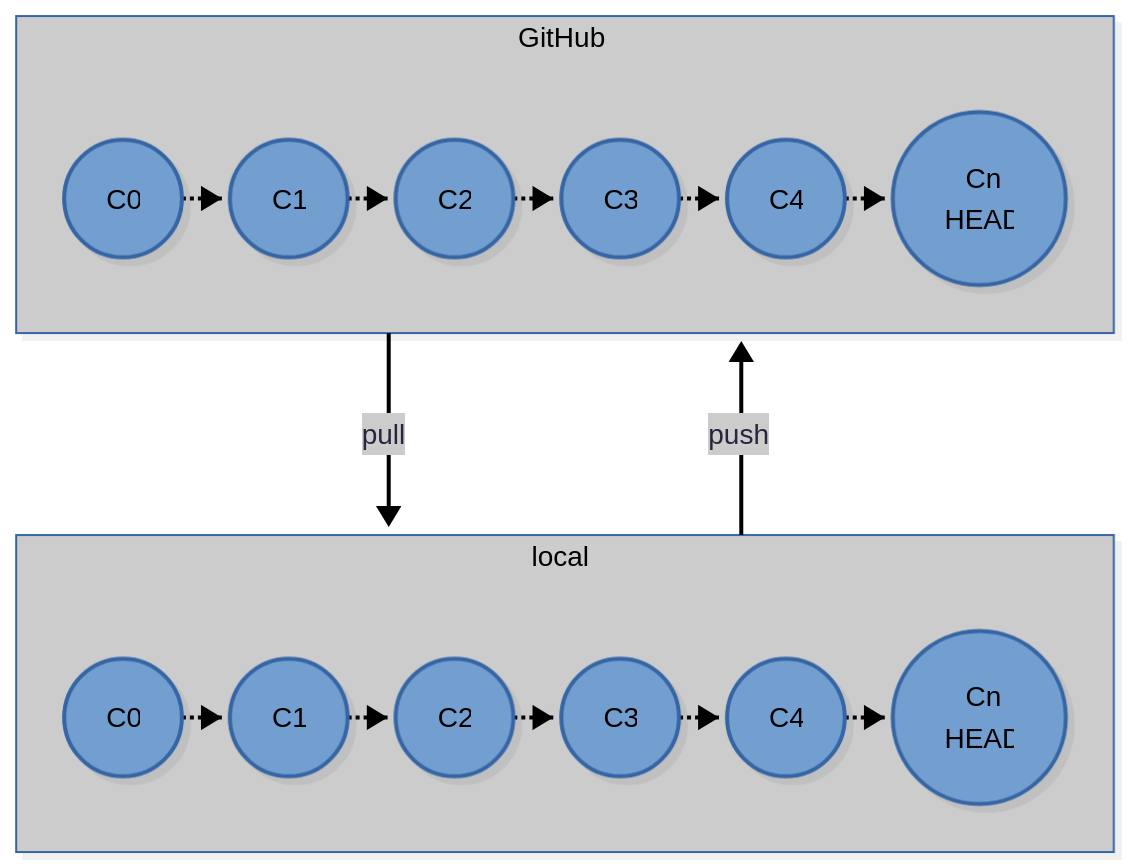
\includegraphics[height=0.8\textheight]{02_local_remoto}
	\end{frame}


\end{document}
